\section{Shark Attack}
\label{sec:shark_attack}	

\subsection*{Recommended Tutorials:}
\begin{itemize}[noitemsep]
	\item \nameref{chp:assignment_operator}, pg. \pageref{chp:assignment_operator}
	\item \nameref{chp:equation_solvers}, pg. \pageref{chp:equation_solvers}
	\item \nameref{chp:definite_and_indefinite_Integrals}, pg. \pageref{chp:definite_and_indefinite_Integrals}
\end{itemize}

\subsection*{Introduction:}

In this activity, you will determine whether you can swim to safety before a shark attacks. You will need to use piecewise functions and the Net Change Theorem to find the outcome. 

\tikzset{
   ragged border/.style={ decoration={random steps, segment length=1mm, amplitude=0.5mm},
           decorate,
   }
}
\begin{figure}[h]
\centering
\begin{tikzpicture}
    \fill[cyan!30] decorate[ragged border]{ (0,2) -- (8,2) } -- (8,0) -- (0,0) -- cycle;
    \fill[yellow!30] decorate[ragged border]{ (8,2) -- (8,0) } -- (9,0) -- (9,2) -- cycle;
    \draw (1.5,1) node {\scalebox{-0.2}[0.2]{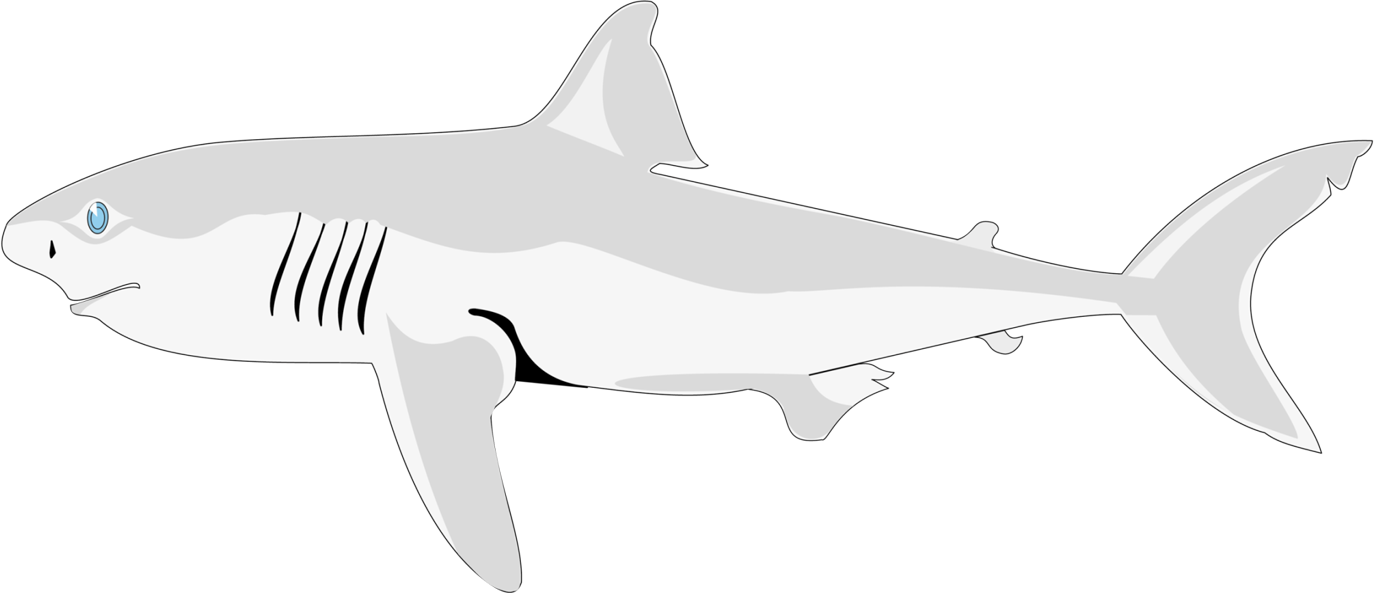
\includegraphics{activities/math122/figures/shark.png}}};
    \draw (5,1) node {
\includegraphics[scale=0.075]{activities/math122/figures/swimmer.png}};
    \draw[|-|] (1.5,3) node [above] {$\SI{0}{m}$} -- (5,3) node [above] {$\SI{50}{m}$};
    \draw[|-|] (5,3) -- (8,3) node [above] {$\SI{70}{m}$};
\end{tikzpicture}
\caption{An illustration of the shark trying to catch you as you swim to shore.}
\label{fig:shark_attack}
\end{figure}

Suppose that you are surfing on the ocean and there is a shark $\SI{50}{m}$ behind you, at rest (i.e. $v(0)=0$). \\

The shark senses you and begins accelerating toward you at a rate of $\SI{5}{m/s^2}$, up to a top speed of $\SI{13}{m/s}$.
You see the shark coming and begin swimming towards shore at a speed of $\SI{2}{m/s}$. Assume there is no time needed for you to accelerate up to your top speed. If the shore is $\SI{20}{m}$ away from you (and $\SI{70}{m}$ away from the shark), do you make it to shore before the shark attacks?

\begin{marginfigure}[-2cm]
\centering
\begin{tikzpicture}
\begin{axis}[
	width=\textwidth,
	height=0.8\textwidth,
	clip=false,
	axis lines=middle,
	xlabel={$t$},
	ylabel={$v$},
	xlabel style={below right},
	ylabel style={above left},
	xmin=-0.5, xmax=8, xtick={0},
	ymin=-2, ymax=15, ytick={0,13}
]
	\addplot [domain=0:2.6, samples=100] {5*x};
	\addplot [domain=2.6:8, samples=100] {13};
	\draw [dashed] (axis cs:2.6,13) -- (axis cs:2.6,0);
	\draw (axis cs:2.6,0) node [below] {$t_1$};
\end{axis}
\end{tikzpicture}
\caption{The shark speeds up to its top speed of $\SI{13}{m/s}$ with a constant acceleration of $\SI{5}{m/s^2}$. This results in a piecewise defined function $v(t)$ shown here.}
\label{fig:sharkvelocity}
\end{marginfigure}

\subsection*{Exercises:}

\begin{enumerate}
    \item Calculate the time $t_1$ it takes for the shark to reach its top speed of $13$ m/s if it accelerates at $5$ m/s\textsuperscript{2}. Note that the shark will no longer accelerate after $t_1$ seconds, since it has reached its top speed. \label{ex:sharktime}
    \marginnote[-1.5cm]{The shark's velocity will contain an acceleration term for $0 \le t \le t_1$ (where $t_1$ is the time you find in exercise \ref{ex:sharktime}) but will not have an acceleration term after $t_1$ seconds.}
    \item Define a piecewise function for the shark's velocity using the \texttt{piecewise()} command and assign this to $sharkvelocity(t)$. This velocity function should be linearly increasing if $0 \leq t \leq t_1$ and constant if $t > t_1$.
    \marginnote[-0.5cm]{You can read how to define piecewise functions on page \pageref{sec:piecewise}.}
    \index{mathematical functions!piecewise}
    \item Integrate $sharkvelocity(t)$ to find the distance function for the shark.
    \item Since your velocity is constant at $2$ m/s, assign the function $swimvelocity(t) = 2$.
    \item Integrate $swimvelocity(t)$ to find your distance function. 
    \marginnote[1.5cm]{Try using the \texttt{solve()} command first, then change it to \texttt{fsolve()} if necessary.}
    \index{solving equations!solve}\index{solving equations!fsolve}
    \item Since you start $50$ m ahead of the shark ($d(0)=50$), add the $50$ m to your distance function and set this equal to the distance function for the shark. Solve this equation to find the total time required for the shark to catch up to you.
    \marginnote[0.5cm]{For convenience, we will let the shark's initial position be $0$ m and your initial position be $50$ m. This means the shore is at a position of $70$ m.}
    \item Plug this time into the shark's distance formula to determine the distance the shark travels while it is pursuing you. Will you make it to the shore safely? Explain your answer in a new paragraph.
    \marginnote[1cm]{You may wish to specify colours for each function so that you can tell which function is which.}
    \item Plot the distance functions for you and the shark on the same graph. Be sure to include your $50$ m head start in your distance function. Adjust your plot so that you can see the moment that the shark catches up to you.
    \item Instead of swimming, let's suppose you surf the nearest wave away from the shark, accelerating you at $2$ m/s$^2$. Starting from rest, the wave accelerates you to a top speed of $4$ m/s. Define a new piecewise function and assign it to $surfvelocity(t)$. Repeating your previous steps, determine the distance that the shark must travel before it catches you. Will you make it to the shore safely?
    \marginnote[-1cm]{In this case, your surfing velocity function will be similar to the shark's velocity function.}
\end{enumerate}